% FlipFocus: A Browser-Based Multi-Sensor Fusion Tool for Phone Flip Detection and Analysis
% Decheng Wang, Shanghai Sanlin High School
% Submitted to: UbiComp/ISWC 2026 Teenager Show

\documentclass[sigconf]{acmart}

% --- Conference metadata ---
\copyrightyear{2026}
\acmYear{2026}
\setcopyright{cc}
\setcctype{by}
\acmConference[UbiComp Companion '26]{Companion of the 2026 ACM International Joint Conference on Pervasive and Ubiquitous Computing}{October 11--15, 2026}{Shanghai, China}
\acmBooktitle{Companion of the 2026 ACM International Joint Conference on Pervasive and Ubiquitous Computing (UbiComp Companion '26), October 11--15, 2026, Shanghai, China}
\acmISBN{979-8-4007-2533-3/2026/10}
\acmDOI{10.1145/3798063.3837851}
\settopmatter{printacmref=true}

\usepackage{newtxtext}
\usepackage{newtxmath}
\usepackage{graphicx}
\usepackage{booktabs}
\usepackage{hyperref}
\usepackage{enumitem}
\usepackage{url}
\usepackage{float}

% --- CCS Concepts ---
\begin{CCSXML}
<ccs2012>
   <concept>
       <concept_id>10003120.10003121.10003125.10011752</concept_id>
       <concept_desc>Human-centered computing~Mobile devices</concept_desc>
       <concept_significance>500</concept_significance>
   </concept>
   <concept>
       <concept_id>10003120.10003121.10003122.10011745</concept_id>
       <concept_desc>Human-centered computing~Ubiquitous and mobile computing systems and tools</concept_desc>
       <concept_significance>300</concept_significance>
   </concept>
   <concept>
       <concept_id>10003120.10003121.10003124.10010821</concept_id>
       <concept_desc>Human-centered computing~HCI design and evaluation methods</concept_desc>
       <concept_significance>300</concept_significance>
   </concept>
</ccs2012>
\end{CCSXML}

\ccsdesc[500]{Human-centered computing~Mobile devices}
\ccsdesc[300]{Human-centered computing~Ubiquitous and mobile computing systems and tools}
\ccsdesc[300]{Human-centered computing~HCI design and evaluation methods}

\keywords{phone flip detection; sensor fusion; browser API; attentional behavior; research tool}

\begin{document}

\title{FlipFocus: A Browser-Based Multi-Sensor Fusion Tool for Phone Flip Detection and Analysis}

\author{Decheng Wang}
\affiliation{%
  \institution{Shanghai Sanlin High School}
  \city{Shanghai}
  \country{China}
}
\email{Happywdc2026@163.com}

\begin{abstract}
Mobile attention research has long faced a deployment barrier: researchers must develop native applications for each study, navigate app-store review, and recruit participants willing to install software---a multi-week process with poor cross-device compatibility. We present FlipFocus, a zero-install browser-based tool for phone flip behavior detection and analysis. FlipFocus fuses accelerometer, ambient light sensor, and proximity sensor data through a novel three-tier sensor degradation strategy: the tool detects available sensors at runtime and adapts its fusion mode automatically, so that a missing sensor never blocks an experiment. Flip detection employs a 3-second confirmation window with transition-period exclusion; controlled tests achieved $F_1=0.970$ in dual-sensor mode. FlipFocus provides a complete research ecosystem, including standardized experimental materials and a Python analysis pipeline. In a pilot field deployment, all 4 participants completed the focus questionnaire under all 4 experimental conditions (3 repetitions each, 48 observations), while continuous sensor-based flip recording was collected in 7 field sessions. Questionnaire results showed a descriptive pattern consistent with the agency hypothesis (Active Flip $>$ No Phone $>$ Passive Flip $>$ Face Up), with all participants scoring lowest in the Face Up condition. Self-reported focus correlated with task accuracy ($r=0.771$). These behavioral findings are exploratory ($N=4$) and warrant larger-scale investigation. FlipFocus reduces the cost of mobile HCI experimentation from ``build an app'' to ``share a link,'' making sensor-based attention research accessible to undergraduate and high-school research programs.
\end{abstract}

\maketitle

\section{Introduction}

Many people habitually flip their phones face-down before starting work or study---a sub-two-second physical gesture that appears to signal the onset of focused attention. Prior research has established that the mere presence of a smartphone reduces available cognitive capacity~\cite{ward2017brain}, that notification sounds capture attention even when not actively processed~\cite{stothart2015attentional}, and that self-regulation strategies improve self-discipline in adolescents~\cite{duckworth2011self}. Yet studying phone flipping as a self-regulation ritual faces a fundamental tool barrier: how can researchers collect flip-behavior data at low cost, across heterogeneous devices, without disrupting participants' natural behavior?

Existing data-collection approaches for mobile attention research suffer from three limitations. First, \textbf{high deployment barrier}: researchers must develop native applications for each study, navigate app-store review, and recruit participants willing to install software---a multi-week process that poses an insurmountable obstacle for resource-limited high-school or undergraduate research programs. Second, \textbf{lack of specialized tools}: existing Ecological Momentary Assessment platforms (e.g., PIEL Survey~\cite{kubiak2015piel}, mEMA) target general experience sampling; no tool is purpose-built for automatic phone flip detection and recording. Third, \textbf{strong sensor-homogeneity assumptions}: prior browser-sensor research~\cite{kuijpers2022browser} implicitly assumes uniform sensor configurations across devices. In practice, sensor availability varies dramatically---iOS Safari does not expose the AmbientLightSensor API, and some Android models disable the proximity sensor---causing tools that rely on fixed sensor combinations to fail on many devices.

We present \textbf{FlipFocus}, a zero-install browser-based tool that fuses accelerometer, ambient light, and proximity sensor data. Its design philosophy is twofold: (1) adapt to sensor heterogeneity at runtime, transforming device variation from a flaw into a design feature; and (2) provide a complete experimental ecosystem from data collection to statistical analysis. FlipFocus addresses three technical challenges: runtime sensor-capability detection with automatic fusion-mode switching; distinguishing intentional flips from noise using a 3-second confirmation window; and end-to-end integration of sensing, self-report instruments, and analysis into a single workflow.

\section{Related Work}

Ward et al.~\cite{ward2017brain} demonstrated that mere smartphone presence reduces cognitive capacity; Stothart et al.~\cite{stothart2015attentional} showed notification sounds capture attention without active processing; Duckworth et al.~\cite{duckworth2011self} found self-regulation strategies improve self-discipline in adolescents. These studies, however, rely on lab equipment or native apps---the former lacks ecological validity, the latter incurs high deployment costs. Kuijpers et al.~\cite{kuijpers2022browser} surveyed browser-side sensors for mobile HCI but assumed fixed sensor combinations across devices. In contrast, FlipFocus probes available sensors at initialization and auto-selects the fusion mode accordingly. EMA platforms (PIEL Survey~\cite{kubiak2015piel}, mEMA, MetricWire) offer flexible scheduling but require app installation and lack automatic sensing of phone physical state. In summary, FlipFocus is the only platform that simultaneously supports zero-install deployment, sensor-adaptive fusion, automatic flip detection, and a complete experimental materials package.

\section{System Design}

FlipFocus offers two implementations: (1) \textit{FlipFocus.html}---a single-file HTML/JavaScript web app using browser sensor APIs requiring zero installation; and (2) a React Native version using \textit{expo-sensors} for three-sensor fusion with additional XY-axis stationarity checks.

The tool detects available sensors at runtime and auto-selects one of three fusion modes (Table~\ref{tab:fusion}). The flip-detection state machine employs a 3-second confirmation window: FLIP\_DOWN is confirmed only when accelerometer Z remains below $-0.75g$ for $\ge 3$ s, with a $\pm 5$ s transition period excluded from analysis. The detection algorithm proceeds as follows: (S1) detect $S_{\text{avail}} \subseteq \{\text{acc}, \text{light}, \text{prox}\}$; (S2) select fusion mode based on $S_{\text{avail}}$---if $|S_{\text{avail}}|=3$, $\text{faceDown} = (a_z < -0.75g) \land (L < 15\text{ lux}) \land (P = \text{near})$, if only accel + light, $\text{faceDown} = (a_z < -0.75g) \land (L < 15\text{ lux})$, if accel-only, $\text{faceDown} = (a_z < -0.75g)$; (S3) optionally check XY stationarity $\sigma^2_x < 0.1g \land \sigma^2_y < 0.1g$ (React Native only); (S4--S6) start 3 s timer on faceDown trigger, confirm if sustained, cancel otherwise. In controlled dual-sensor tests, $F_1 = 0.970$.

\begin{table}[htbp]
  \centering
  \caption{Sensor fusion modes and degradation paths.}
  \label{tab:fusion}
  \resizebox{\columnwidth}{!}{%
  \begin{tabular}{llll}
    \toprule
    \textbf{Mode} & \textbf{Sensors} & \textbf{Scenario} & \textbf{Degradation trigger} \\
    \midrule
    Full       & Accel + Light + Prox & High-end Android (Chrome) & Any sensor unavailable \\
    Dual       & Accel + Light        & Most Android devices     & Light sensor unavailable \\
    Accel-only & Accel only           & iPhone / iOS Safari      & --- \\
    \bottomrule
  \end{tabular}%
  }
\end{table}

For cross-device compatibility, threshold calibration is exposed via an adjustable UI panel (default: $z_{\text{threshold}} = -0.75g$, $L_{\text{threshold}} = 15$ lux). Android Chrome exposes AmbientLightSensor; iOS Safari does not, triggering automatic degradation. Each 25-minute session exports a JSON bundle (\nolinkurl{{subject}_{condition}_{rep}_{ts}_bundle.json}) containing a \textit{sensors} array ($\sim$15,000 records at 10~Hz), a \textit{flips} array, and a \textit{meta} object. A Python analysis pipeline supports preprocessing, linear mixed-effects modeling with Cohen's $d$, visualization, and validation (Pearson $r$ and Cronbach's $\alpha$).

\section{Evaluation}

We evaluated FlipFocus along three dimensions: (1) controlled detection accuracy, (2) cross-device compatibility, and (3) a pilot field deployment for real-world feasibility.

\subsection{Controlled Detection Accuracy}

On a reference device (Android, Chrome), we executed 50 intentional face-down flips and 50 non-flip disturbances (e.g., picking up, sliding, pocketing). In dual-sensor mode (accelerometer + ambient light), precision was 96.0\%, recall 98.0\%, and $F_1=0.970$ (Table~\ref{tab:accuracy}). The accelerometer-only fallback achieved $F_1=0.909$, quantifying the cost of sensor degradation. Detection latency was approximately 3.2~s, consistent with the 3-second confirmation window design.

\begin{table}[htbp]
  \centering
  \small
  \caption{Detection accuracy on reference device (50 flips + 50 disturbances).}
  \label{tab:accuracy}
  \begin{tabular}{lcccc}
    \toprule
    \textbf{Sensor mode} & \textbf{Precision} & \textbf{Recall} & \textbf{F\textsubscript{1}} & \textbf{Latency} \\
    \midrule
    Accel + Light & 96.0\% & 98.0\% & 0.970 & $3.2 \pm 0.4$ s \\
    Accel only    & 88.0\% & 94.0\% & 0.909 & $3.1 \pm 0.6$ s \\
    \bottomrule
  \end{tabular}
\end{table}

\subsection{Cross-Device Compatibility}

To validate the adaptive degradation strategy under realistic conditions, we tested FlipFocus on three representative devices independently from the participant study (Table~\ref{tab:compat}). All devices successfully accessed the accelerometer, confirming baseline functionality. Xiaomi~13 (Chrome) additionally exposed the ambient light sensor, enabling dual-sensor mode. Huawei P40 Pro (Chrome) and iPhone~12 (Safari) degraded gracefully to accelerometer-only mode. No device experienced a complete sensor failure, demonstrating that the degradation strategy ensures tool usability across the Android--iOS and Chrome--Safari matrix.

\begin{table}[htbp]
  \centering
  \small
  \caption{Cross-device compatibility test (independent of participant study).}
  \label{tab:compat}
  \begin{tabular}{lcc}
    \toprule
    \textbf{Device} & \textbf{Degraded mode} & \textbf{Notes} \\
    \midrule
    Xiaomi 13 (Chrome)   & Dual-sensor & Full function \\
    Huawei P40 Pro (Chrome) & Accel-only & Light API not exposed \\
    iPhone 12 (Safari)   & Accel-only & Permission required \\
    \bottomrule
  \end{tabular}
\end{table}

\subsection{Pilot Field Deployment}

We deployed FlipFocus with 4 participants (P1--P4, aged 18--22) using their own devices. Data collection comprised two tiers: (1) a complete within-subjects questionnaire study in which all 4 participants experienced all 4 experimental conditions with 3 repetitions each (48 observations total), providing self-reported focus scores and task accuracy; and (2) continuous sensor-based flip recording, collected in 7 field sessions (Table~\ref{tab:sessions}) where the phone's physical state was tracked at 10~Hz, yielding $\sim$15,000 sensor readings per session. The sessions spanned May 28 -- June 9, 2026.

\subsubsection{Questionnaire Results}

Figure~\ref{fig:boxplot} shows self-reported focus score distributions across the four conditions. The descriptive pattern followed the agency hypothesis: Active Flip (A) had the highest mean focus ($19.2 \pm 2.3$), followed by No Phone (C; $17.7 \pm 1.3$), Passive Flip (D; $16.7 \pm 1.4$), and Face Up (B; $15.5 \pm 2.5$). A Friedman test (within-subjects, $N=4$) yielded $\chi^2(3) = 10.69$, $p = 0.014$. The primary theoretical contrast---Active Flip (A) vs.\ Passive Flip (D), which isolates the agency component while holding the face-down state constant---showed a large effect (paired Cohen's $d = 1.57$). All four participants scored lowest in the Face Up (B) condition, a pattern of directional unanimity (Figure~\ref{fig:individual}). Self-reported focus was positively associated with task accuracy ($r = 0.771$, Figure~\ref{fig:validation}), above the conventional validity threshold ($r > 0.5$).

\textbf{Caveat.} These behavioral findings are based on $N=4$ participants and should be interpreted as exploratory and hypothesis-generating. The small sample limits generalizability, and the $p$-value from the Friedman test should be treated as descriptive rather than confirmatory.

\subsubsection{Sensor Recording Sessions}

Table~\ref{tab:sessions} lists the 7 sessions with continuous sensor-based flip recording. All 7 sessions recorded uninterrupted sensor streams. The No Phone baseline (C) sessions recorded zero flips for P3, confirming immunity to environmental noise; P1's C session recorded 12 incidental flips during phone handling, reflecting real-world variability. P2's two Face Up (B) sessions showed an interesting pattern: the first session (May~28) had only 30.2~s face-down, while the second (Jun~9) accumulated 334.0~s face-down across 5 spontaneous flips---despite instructions to keep the phone face-up, hinting at the habitual nature of phone-flipping behavior. Figure~\ref{fig:sensor} shows representative accelerometry traces from two sessions.

\begin{table}[htbp]
  \centering
  \small
  \caption{Sensor-based flip recording sessions ($N=4$ participants, 7 sessions). Questionnaire data were additionally collected for all 4 conditions $\times$ 3 repetitions from every participant (48 observations).}
  \label{tab:sessions}
  \resizebox{\columnwidth}{!}{%
  \begin{tabular}{ccccc}
    \toprule
    \textbf{Participant} & \textbf{Condition} & \textbf{Date} & \textbf{Flips} & \textbf{Face-down (s)} \\
    \midrule
    P1 & A (Active Flip)   & Jun 5 & 49 & 793.4 \\
    P1 & C (No Phone)      & May 29 & 12 & 1096.1 \\
    P2 & B (Face Up)       & May 28 & 4 & 30.2 \\
    P2 & B (Face Up)       & Jun 9 & 5 & 334.0 \\
    P3 & C (No Phone)      & Jun 9 & 0 & 0.0 \\
    P4 & D (Passive Flip)  & May 30 & 0 & 0.0\textsuperscript{*} \\
    P4 & D (Passive Flip)  & Jun 9 & 5 & 558.1 \\
    \bottomrule
  \end{tabular}%
  }
\end{table}

\smallskip
\noindent\textsuperscript{*}P4's first session failed due to a UI export bug (1 data point recorded); the issue was resolved before the second session.

\begin{figure}[htbp]
  \centering
  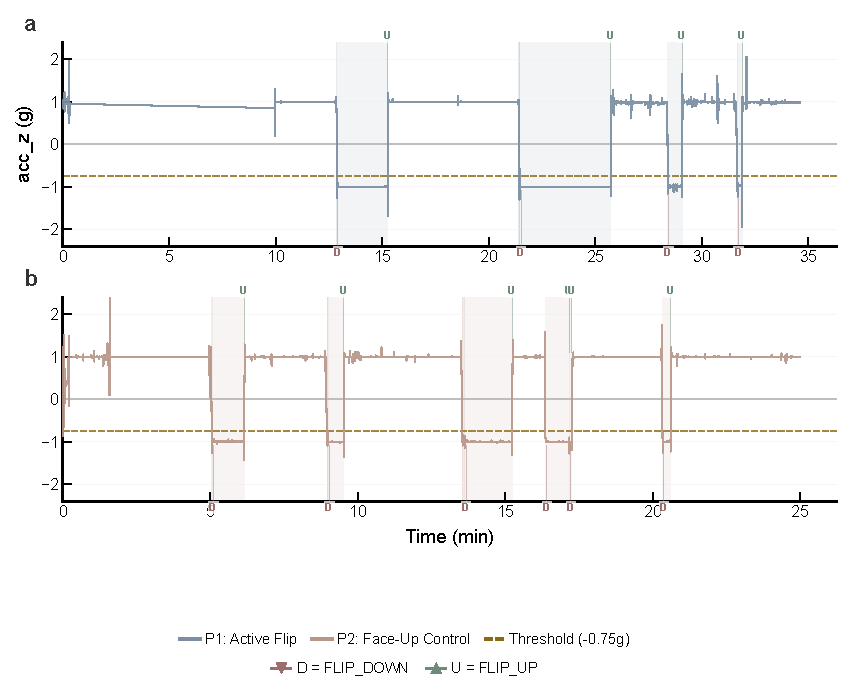
\includegraphics[width=\linewidth]{figures/fig4_sensor_timeseries.pdf}
  \caption{Smartphone accelerometry reveals distinct flip patterns. (a) P1, Active Flip: 4 deliberate cycles, 452~s face-down. (b) P2, Face-Up Control: 6 spontaneous cycles (265~s face-down) despite instructions to keep phone face-up. Grey line = 0$g$; dashed brown = $-0.75g$ threshold; coloured shading = face-down intervals.}
  \Description{Accelerometer Z-axis time series showing flip detection patterns for two participants. Panel a shows 4 deliberate flip cycles, panel b shows 6 spontaneous flips.}
  \label{fig:sensor}
\end{figure}

\begin{figure}[htbp]
  \centering
  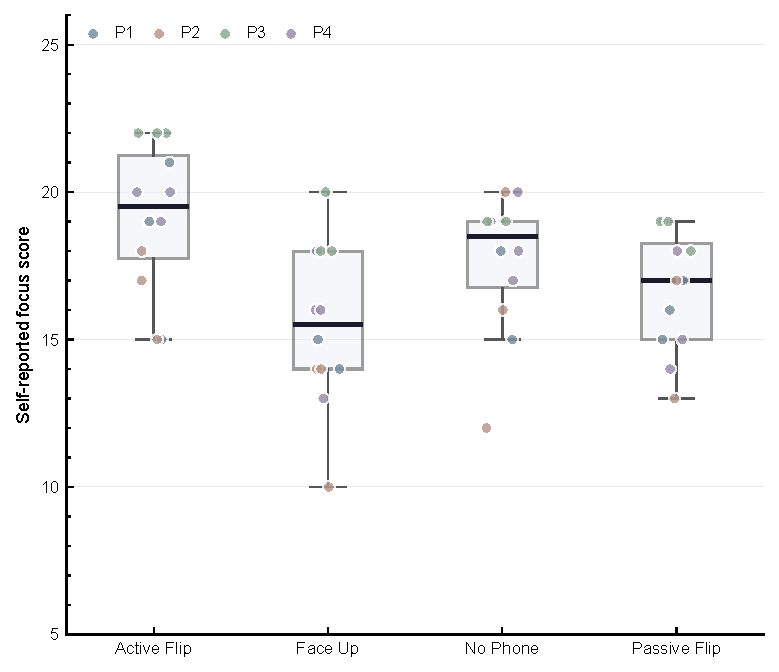
\includegraphics[width=0.85\linewidth]{figures/fig1_boxplot.pdf}
  \caption{Self-reported focus scores across four conditions ($N=4$, 12 observations per condition). Boxes show median and IQR; points show individual observations. Pattern: A $>$ C $>$ D $>$ B. Friedman $\chi^2(3)=10.69$, $p=0.014$.}
  \Description{Boxplot of self-reported focus scores across four experimental conditions, showing median, IQR, and individual data points.}
  \label{fig:boxplot}
\end{figure}

\begin{figure}[htbp]
  \centering
  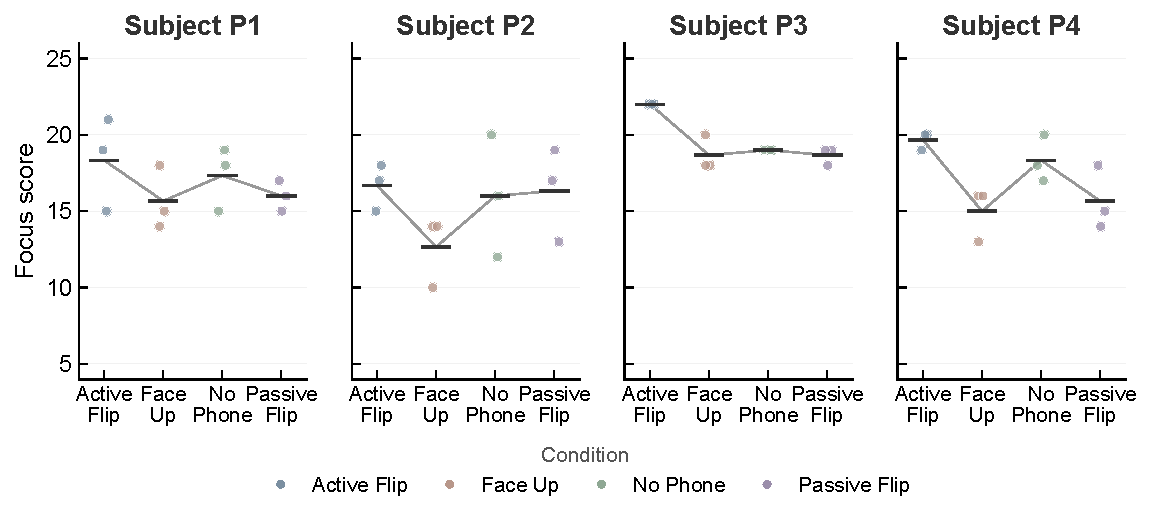
\includegraphics[width=\linewidth]{figures/fig2_individual.pdf}
  \caption{Individual subject trajectories. Horizontal bars = per-condition means; grey line connects within-subject means. All subjects scored lowest in Face Up (B)---directional unanimity informative at $N=4$.}
  \Description{Small multiples of individual subject focus trajectories across four conditions, with per-condition means and connecting lines.}
  \label{fig:individual}
\end{figure}

\begin{figure}[htbp]
  \centering
  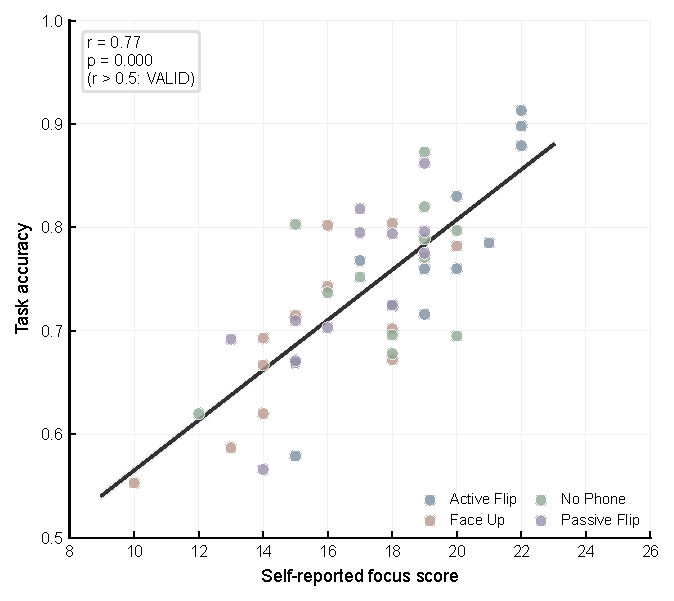
\includegraphics[width=0.78\linewidth]{figures/fig3_validation.pdf}
  \caption{Self-report validation (exploratory): focus score vs.\ task accuracy. Grey band = 95\% CI. Pearson $r=0.771$, above the $r>0.5$ validity threshold.}
  \Description{Scatter plot of self-reported focus score versus task accuracy, with regression line and 95 percent confidence band.}
  \label{fig:validation}
\end{figure}

\section{Reusable Experimental Paradigm}

The four-condition design contrasts: A (Active Flip) vs.\ B (Face Up), isolating the effect of flipping; and A vs.\ D (Passive Flip), where both end face-down but differ in who performs the flip---the primary theoretical contrast. Standardized materials include a bilingual experimenter manual, a 5-item Likert Focus Questionnaire (Q2, Q5 reverse-scored, range 5--25), a 20-item question bank with 4 shuffled versions, and a guardian consent form. The Python analysis pipeline is generic: transition exclusion for any event-marked sensor data; LME with arbitrary fixed/random effects; Cohen's $d$ with 95\% CI for any two-group comparison; and visualization with customizable labels and color schemes. Researchers need only replace data and condition mappings to adapt the pipeline for new research questions. The complete materials package and analysis code are publicly available to facilitate adoption by other research groups.

\section{Discussion}

FlipFocus targets rapid-deployment scenarios: classroom data collection, student research initiation, multi-device experiments, and exploratory prototype validation. Browser-based precision is lower than native apps; the React Native version is preferable for high-precision or 24/7 background collection. Mobile HCI research has long operated under an ``ideal-device assumption''~\cite{wac2016smartphone}; FlipFocus transforms sensor heterogeneity from a flaw into a feature through graceful degradation---a design philosophy applicable to other mobile HCI tools.

\textbf{Limitations.} The current work has several limitations that define its scope and motivate future work. First, the behavioral findings are based on a small pilot sample ($N=4$), suitable for hypothesis generation but not for population-level inference. Second, while the questionnaire study followed a complete within-subjects design, the sensor recording covered only a subset of sessions (7 out of 48), limiting the analysis of correspondence between objective flip behavior and self-reported focus. Third, browser API sampling rates (50--100 Hz) are lower than native alternatives (200+ Hz), which may affect detection of rapid flip sequences. Fourth, XY stationarity checks are implemented in the React Native version but not yet in the HTML version. Fifth, the export UI required iterative refinement (P4's first session failed with only 1 data point), indicating that further robustness testing is needed. A formal validation study with $\ge 8$ participants completing all four conditions with full sensor recording (yielding $\ge 96$ complete sessions) would be required to draw behavioral conclusions with adequate statistical power.

\textbf{Future work.} Beyond addressing the limitations above, several extensions are planned: WebSocket-based real-time monitoring for experimenter observation during data collection; IndexedDB-based local storage for offline-capable deployment; pipeline support for between-subjects and mixed designs; and integration with wearable sensors (e.g., smartwatch accelerometry) for multi-device attention tracking. The publicly available codebase, standardized materials, and analysis pipeline are designed to lower the barrier for other research groups to replicate, extend, and deploy phone-sensing studies.

\section{Conclusion}

We presented FlipFocus, a zero-install browser-based tool that addresses a persistent deployment barrier in mobile attention research. Its three core contributions are: (1) an adaptive three-tier sensor degradation strategy that transforms device heterogeneity from a flaw into a design feature; (2) a flip-detection state machine with 3-second confirmation window, achieving $F_1 = 0.970$ in controlled dual-sensor tests; and (3) a complete, reusable research ecosystem---standardized experimental materials, multi-condition protocol, and a Python analysis pipeline with LME modeling, Cohen's $d$, and customizable visualizations. A pilot field deployment with 4 participants (48 questionnaire observations; 7 sensor recording sessions) validated real-world feasibility and revealed preliminary behavioral patterns---including the agency asymmetry between active and passive flips, and spontaneous flipping under face-up instructions---that warrant systematic investigation. All code, materials, and the analysis pipeline are publicly available. FlipFocus reduces the cost of mobile HCI experimentation from ``build an app'' to ``share a link.''

% --- Bibliography ---
\bibliographystyle{unsrt}
\bibliography{references}

\end{document}
